%----------------------------------------------------------------------------------------

% Define some commands to keep the formatting separated from the content 
\newcommand{\keyword}[1]{\textbf{#1}}
\newcommand{\tabhead}[1]{\textbf{#1}}
\newcommand{\code}[1]{\texttt{#1}}
\newcommand{\file}[1]{\texttt{\bfseries#1}}
\newcommand{\option}[1]{\texttt{\itshape#1}}
\newcommand{\grados}{$^{\circ}$}

%----------------------------------------------------------------------------------------
%\section{Introducción}
%----------------------------------------------------------------------------------------

% Chapter 1

\chapter{Introducción} % Main chapter title
\label{Chapter1} % For referencing the chapter elsewhere, use \ref{Chapter1} 
\label{Intro}

Los sistemas de información visual para pasajeros están presentes en diversas industrias y aplicaciones. Se encargan de proveer información a pasajeros en  movimiento y tienen un rol fundamental en la industria del transporte.\\

 Las personas se trasladan por tierra o aire usando automóviles, ómnibus, subtes, trenes o aviones, entre otros. Los sistemas de información visual para cada cada caso presentan necesidades y soluciones distintas. En una autopista se suele comunicar accidentes u obras viales en ejecución a los conductores a través de carteles gigantes y con información en tiempo real. En los aeropuertos los pasajeros visualizan la información de arribo, estado o despegue de  vuelo. A los pasajeros de ómnibus les interesa conocer los tiempos de espera y las líneas en operación al llegar a una estación. En un caso los carteles pueden estar a la intemperie y en  otro dentro de un recinto, pero siempre requieren estar sincronizados con los vehículos en movimiento. Los pasajeros de trenes usan estos sistemas para conocer el destino o la próxima estación cuando están viajando. \\

Los sistemas de información al pasajero (PIDS) tienen principalmente tres componentes: un sistema que genera datos, una red de transmisión y un sistema de displays. Dependiendo del dominio de aplicación, las especificaciones de cada sistema tienen distintos requerimientos. Típicamente en los trenes se requiere comunicación en tiempo real, lo que conlleva la adopción de protocolos de tiempo real (RTP). En aplicaciones ferroviarias también es importante la integridad, disponibilidad y confiabilidad de los datos. Pero también existen otros requerimientos de carácter operativo, como el mantenimiento y la facilidad de instalación. Estos últimos aspectos son esenciales en la operación de una formación ferroviaria y tienen impacto directo en el ciclo de vida de un tren.\\

 Los sistemas PIDS instalados en los trenes se interconectan con una red de comunicaciones del tren (TCN). Esta red TCN sigue un estándar y define tanto interfaces eléctricas como protocolos de datos. A la red TCN se conectan dispositivos para el sensado y control de frenos, de puertas, de monitoreo, entre otros, usando una arquitectura jerárquica de buses de datos. La red TCN representa un estándar robusto, maduro, probado y con gran aceptación internacional. Sin embargo los sistemas PIDS se presentan sin la necesidad de ser compatibles con los estándares de TCN. Existen diversas soluciones comerciales para aplicaciones de entretenimiento por ejemplo, pero se requiere de un trabajo de integración adicional para que funcionen en un tren.\\
 
 En este trabajo se introduce una breve descripción de las redes TCN y su evolución en el tiempo. Para el caso de las formaciones de Trenes Argentinos, que forman el marco de este trabajo, se presenta también el detalle de interconexión TCN-PIDS, el desarrollo de un sistema de control para los carteles led del sistema PIDS y los resultados de las pruebas de campo realizadas. Se ha organizado esta memoria buscando acercar al lector primero los conceptos principales de la aplicación y luego el detalle de diseño del sistema embebido propuesto. \\
  

En el capítulo 1 se introduce al lector a la motivación original del trabajo realizado. Se explica el marco de investigación del que forma parte este proyecto y se presenta el estado del arte en controles de carteles led.\\

En el capítulo 2 se introduce vocabulario técnico específico. Se presenta una descripción del sistema con el foco en la red de comunicaciones TCN, el sistema PIDS, sus interacciones y componentes.\\

En el capítulo 3 se abordan cuestiones de diseño de sistema. Se especifican los requerimientos y casos de uso que se plantean en el espacio problema y también las consideraciones del espacio solución. Se detalla la solución en términos de arquitectura, patrones de software, descripción de componentes e implementación. Se incluye también los planos de los circuitos eléctricos del hardware existente que fueron relevados al realizar este trabajo.\\

En el capítulo 4 se abordan cuestiones relacionadas al entorno real del sistema: visitas técnicas, mediciones realizadas, hardware ad-hoc realizado para las mediciones y un breve análisis de las tramas de datos de la red PIDS existente.\\

En el capítulo 5 se tratan las conclusiones principales del desarrollo, su potencial fabricación en serie y los pasos a seguir para integrar al resto de ramales ferroviarios. En el apéndice de bibliografía se encontrarán las principales referencias técnicas, científicas e institucionales relevantes para este trabajo.\\


\pagebreak
\section{Introducción general}
En este trabajo se desarrolla el sistema de control para carteles de matriz led del sistema de información visual para pasajeros de trenes argentinos. Las formaciones de trenes argentinos cuentan con carteles de matriz led en sus coches y en el frente y contrafrente del tren. Todos los carteles se interconectan a una red de comunicación TCN por la que que viajan datos de distintas fuentes: información de sensores, eventos que indican frenado o cierre de puertas, por citar algunos ejemplos. \\

Los carteles led presentan fallas a lo largo de su ciclo de vida. Esto implica realizar tareas de mantenimiento, reparación o reposición. Si bien existen muchos tipos de carteles led disponibles comercialmente, la integración al sistema de comunicaciones del tren es propietaria del fabricante de trenes. Para el caso de trenes argentinos, el proveedor está radicado en China, haciendo no sólo muy costoso sino también muy lento el proceso de reposición o mantenimiento de equipamiento. El desarrollo local de tecnología para sistemas PIDS es estratégico porque extiende la vida útil de los trenes.\\

%Esta necesidad motiva el desarrollo como búsqueda de autonomía tecnológica en áreas de vacancia que pueden ser cubiertas por el sistema científico-tecnológico nacional.

El desarrollo de un sistema a medida para Trenes Argentinos es el eje de este trabajo. La necesidad que prima es generar y brindar al personal de operaciones de la información necesaria para construir y mantener estos sistemas de información visual al pasajero. Como consecuencia, este trabajo también tiene impacto directo en el pasajero, ya que contribuye a la calidad del servicio.\\


\pagebreak
\section{Objetivos y alcance}

El  marco de este trabajo es un Proyecto de Desarrollo Estratégico (PDE) de la Secretaría de Ciencia y Técnica de la Universidad de Buenos Aires (UBACyT). El PDE se titula PDE\_15\_2020 - "Sistema de monitoreo y gestión de la red TCN en formaciones ferroviarias". Las partes que se involucran y forman parte del equipo de trabajo en este proyecto son el Grupo de Investigación en Calidad y Seguridad de las Aplicaciones Ferroviarias (GICSAFE), creado en 2017 en el marco del Consejo Nacional de Investigaciones Científicas y Técnicas (CONICET) de la República Argentina, y la  Operadora Ferroviaria Sociedad del Estado (SOFSE), también conocida como Trenes Argentinos Operaciones. El proyecto está orientado a cubrir necesidades tecnológicas concretas del sistema ferroviario argentino. Este tipo de proyectos son instrumentos de promoción científico-tecnológica que revalorizan e incrementan el aporte de la Universidad al desarrollo socioproductivo.\\

El objetivo principal de este trabajo es diseñar e implementar un sistema de información visual para pasajeros a bordo del tren. El sistema de información visual para pasajeros existente tiene una parte manual y una automática. Cuando el conductor del tren toma cabina para brindar servicio, programa en una pantalla cuáles van a ser las estaciones cabecera. Los nombres de estas estaciones cabecera se visualizan en las marquesinas del frente y contrafrente del tren, como puede verse en la figura \ref{fig:tren}.

\begin{figure}[ht]
	\centering
	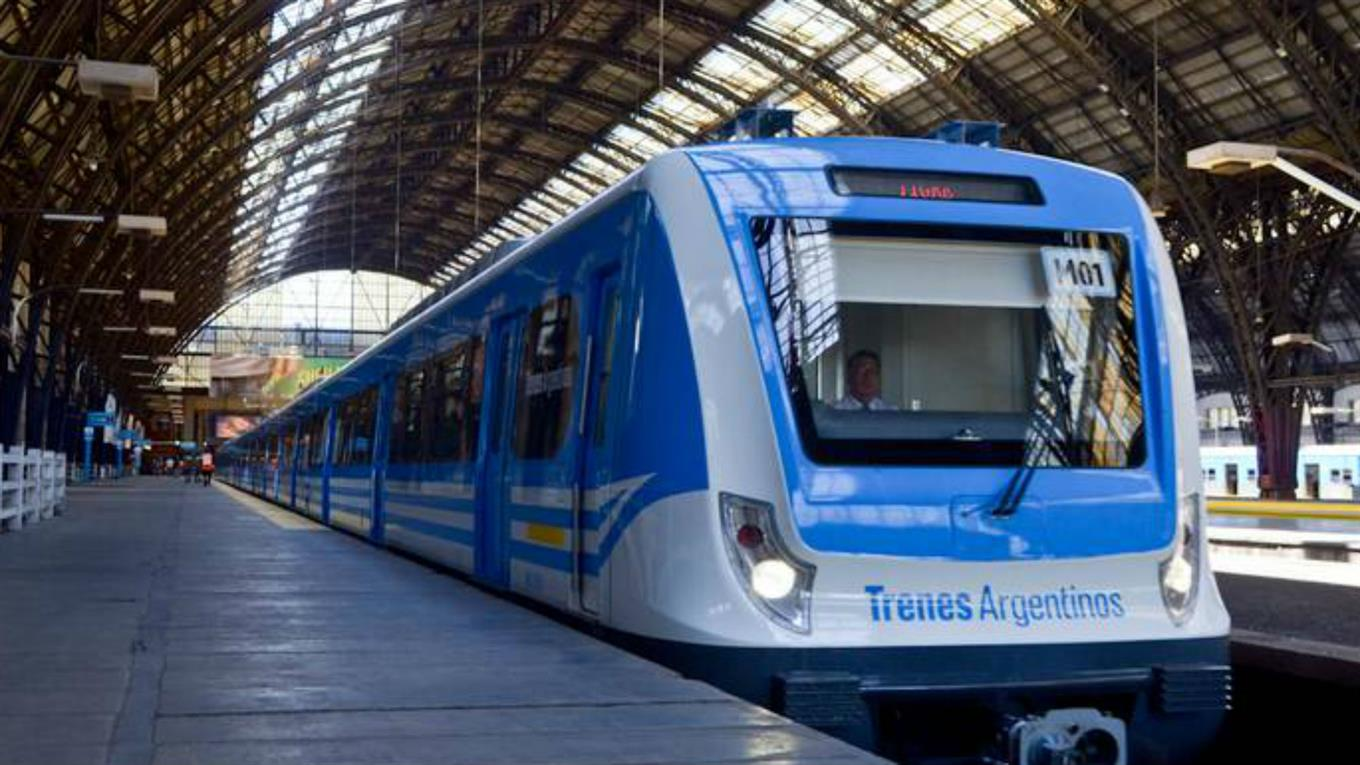
\includegraphics[width=1\textwidth]{./Figures/tren.jpg}
	\caption{Foto de una formación operativa de Trenes Argentinos. Se observa el cartel de matriz led frontal que indica el destino Tigre.}
	\label{fig:tren}
\end{figure}


En el interior de los coches también hay marquesinas led. En estas marquesinas se presentan
mensajes a los pasajeros como el nombre de la próxima estación, o la estación arribada
(“próxima estación Belgrano”, “estás en estación Belgrano”, por ejemplo). Ésta información se
presenta automáticamente en base a variables de sistema que monitorean el detenimiento del
tren, su velocidad y la apertura o cierre de puertas. Esta y otra información de monitoreo y control viaja por una red de comunicación interna del tren que se denomina TCN (Train Communication Network) de acuerdo al estándar que la define [IEC-61375]. Este estándar define para la red TCN dos buses jerárquicos donde se conectan los subsistemas electrónicos: el WTB (Wire Train Bus) [3] y el MVB (Multi-Vehicle Bus) [4]. El primero es el bus de mayor jerarquía que se conecta entre vagones y que se usa para monitorear cambios topográficos del tren. En el
segundo se conectan los sensores y actuadores de cada coche como son los frenos, los controles de puertas, los monitores de velocidad, el sistema de información, etcétera.\\

 El sistema propuesto en este trabajo pretende leer los mensajes de información al pasajero que viajan por la red TCN existente y presentarlos en un display LED. El sistema se compone principalmente de cuatro partes:
 \begin{itemize}
\item display LED
\item placa de control
\item cableado de interconexión
\item firmware del sistema embebido
 \end{itemize}

El diagrama del prototipo se presenta en la figura \ref{fig:diagramaPIDSCIAA}. El display LED matricial representa la marquesina del tren. La placa de control se debe poder conectar al bus MVB de la red TCN como entrada y al display LED como salida.

\begin{figure}[ht]
	\centering
	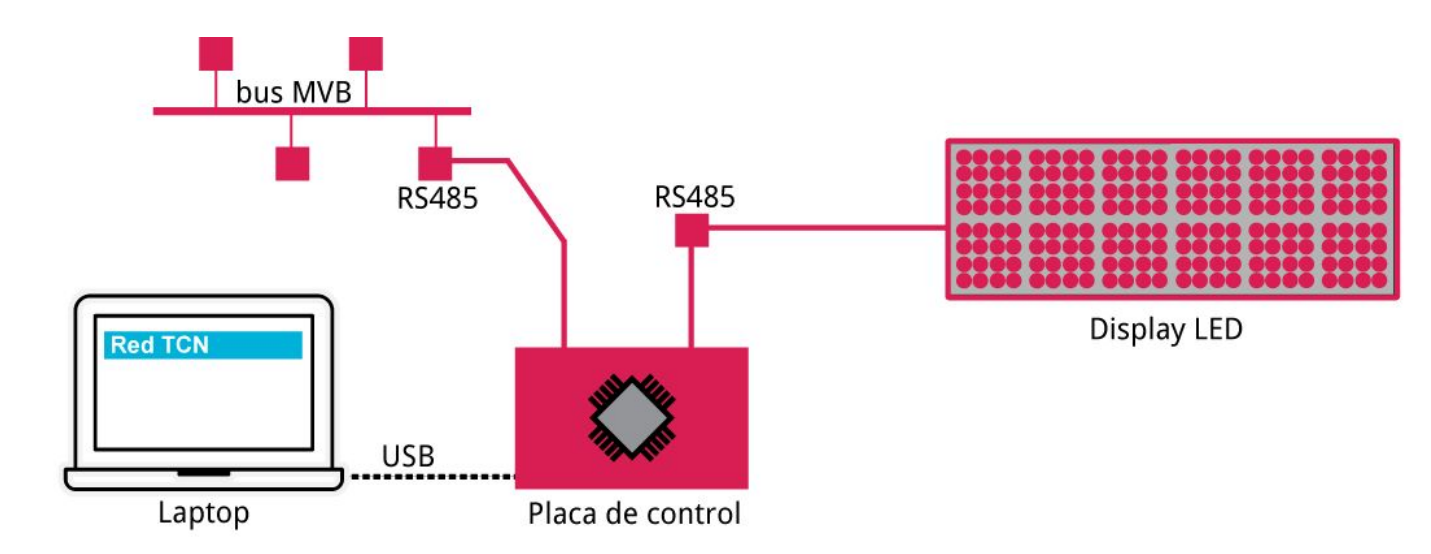
\includegraphics[width=1\textwidth]{./Figures/diagramaPIDSCIAA.png}
	\caption{Diagrama de bloques del sistema embebido propuesto basado en la plataforma EDU-CIAA.}
	\label{fig:diagramaPIDSCIAA}
\end{figure}


La placa de control está basada en alguna de las plataformas desarrolladas por el CONICET-GICSAFe. La conexión entre el display y la placa así como de la placa con la red TCN deberá ser compatible con el estándar RS-485, definido como capa física de la red TCN. El
firmware a desarrollar se carga a la placa de control usando el puerto USB de una laptop. Este firmware es el responsable de leer los mensajes del sistema de información al pasajero y presentarlos en el display.\\

Las cualidades que debe satisfacer este proyecto son:
\begin{itemize}
\item compatibilidad: debe cumplir con los estándares asociados a la red TCN;
\item practicidad: debe ser de fácil uso para el personal de Trenes Argentinos Operaciones
\end{itemize}

Este proyecto permitirá implementar las funciones de visualización del sistema de información al pasajero sin depender del equipamiento existente. El sistema existente es un equipamiento integrado y propietario, y este proyecto busca desacoplar algunas de sus funciones, las que corresponden a la visualización de información, y presentarlas en un display LED genérico. Por otro lado, permitirá reponer los carteles que en la actualidad quedan fuera de servicio por fallas o pérdida del material original y no pueden ser reparados. De esta manera, el valor principal que aporta este proyecto es contribuir con la sustitución de repuestos faltantes por medio de desarrollo y reducir la dependencia tecnológica de la empresa con los fabricantes. Este proyecto tiene impacto directo en las formaciones ferroviarias existentes que brindan servicio al pasajero todos los días.

\pagebreak
\section{Estado del arte}



El cliente de mayor impacto de los servicios que provee un sistema PIDS es la red de transporte (trenes, subtes, metros, ómnibus) de una gran ciudad, debido a su masividad. Lo que se observa en general es que las empresas que proveen sistemas PIDS a las redes metropolitanas de transporte de las grandes ciudades lo hacen bajo formatos distintos. Algunas instalan televisores, otras carteles led, otras incluyen carteles impresos con algún elemento indicador tipo led, leds en forma de flecha para indicar nombres de estaciones impresos, pantallas led para desplegar publicidad entre mensajes, etcétera. En algunos países se han realizado esfuerzos durante la última década para que los sistemas PIDS faciliten el acceso a la información del transporte para personas con discapacidades y de edades avanzadas.


FOTOS

Cuatro principales consideraciones en el abastecimiento de un sistema de información al pasajero son: la disponibilidad de datos ya que su recolección puede requerir uso intensivo de recursos, la precisión de los datos ya que la recolección es susceptible a errores, los mecanismos de entrega de la información al pasajero como puede ser un cartel o una pantalla led, y finalmente la latencia o tiempo de respuesta, donde aparecen soluciones de tiempo real.

[Hitachi] Una vez instalados, los sistemas PIDS suelen requerir mantenimiento. Muchas veces hay fallas de hardware, como por ejemplo leds que dejan de funcionar, una fuente de alimentación o una memoria que se deba reemplazar. Otras veces se requieren cambios en el software, por ejemplo actualizar el contenido de un mensaje o bien cambiarlo. Los atributos de mantenibilidad, versatilidad, modularidad y confiabilidad en la implementación pueden tener un impacto económico relevante en la operación de un servicio de transporte. Para líneas de trenes que cuentan con muchas formaciones ferroviarias operando en simultáneo, las tareas de actualización pueden ser muy intensivas en términos de horas de trabajo y requerir también capacitaciones técnicas periódicas al personal de mantenimiento. Incluso no todos los dispositivos pueden recibir actualizaciones en producción, esto es, en la locación física donde funcionan. Muchas veces se los necesita desinstalar, llevar a un centro técnico y actualizar fuera de operación, lo que requiere de ventanas de mantenimiento y de tiempos reducidos para realizar tareas que pueden ser susceptibles a errores. Otra forma es enviar un técnico al sitio que pueda conectar algún periférico y actualizar manualmente cada dispositivo.

Hitachi ofrece una solución para publicidad de tres pantallas en array que se sincronizan para formar una sola y transmitir video. Cada uno de estos arreglos los posicionan arriba de las ventanas en ambos lados de los coches, alcanzando el despliegue de hasta dieciocho pantallas sincronizadas por coche. Con esto logran transmitir varios mensajes distintos en simultáneo a los pasajeros sin que tengan que moverse de su asiento.

https://www.hitachi.com/rev/archive/2021/r2021\_ 05/05a09/index.html

Toshiba ofrece una solución que permite transmitir publicidad e información al pasajero en una misma pantalla LCD en simultáneo. La solución está centrada en la pantalla como dispositivo central, ofreciendo pantallas de 32" y 42", de 1920 x 540 píxeles, full color de hasta 16.7 millones de colores, de amplio ángulo de visión y de gran luminancia.

https://www.global.toshiba/ww/products-solutions/railway/rolling-stock/passenger-information-display.html
https://www.trapezegroup.com.au/blog/passenger-information-displays-stop-app-website/

Las dimensiones del cartel, la densidad de píxeles por unidad de área, la cantidad de colores o leds por píxel, los niveles de intensidad lumínica, el brillo y contraste, la potencia eléctrica, son algunas de las especificaciones típicas.\\

 Los controladores de los carteles de matriz led suelen basarse en circuitos digitales, en microcontroladores de 8, 16 o 32 bits o en FPGA. La transmisión de datos y el formato de los mismos dependen de la implementación de cada sistema.  \\

En \cite{b1} se utiliza el chip AT89C52 para enviar caracteres chinos sobre matrices de 32 x 192 leds de un solo color; en \cite{b2} se implementa una pantalla led RGB de 320 x 240 píxeles que rota 360º permitiendo visualizar imágenes en color por persistencia de visión; en \cite{b3} se desarrollan algoritmos sobre FPGA usando búferes de datos para controlar una pantalla LED de 160 x 32 píxeles alcanzando 32,768 colores; en \cite{b4} se presenta el control de un micro display de transistores de película delgada (TFT) usando modulación por ancho de pulso (PWM) alcanzando 256 niveles de color a una frecuencia de refresco de 60 Hz, basado también en FPGA; en \cite{b5} se presenta el control de píxeles virtuales para matrices led multicolor usando flip-flops tipo D. \\

En el diseño e implementación del presente trabajo, los carteles son de matriz led de un solo color y de distintas dimensiones (8x64, 32 x 64, 32 x 128). El control de los carteles tiene como factor común el uso del conjunto de chips digitales 74HC138, 74HC595 y 74HC245. La topología permite interconectar paneles en serie para construir carteles led de distinto tamaño usando la misma lógica de control. \\

\pagebreak
\section{Bibliografía}
\label{sec:biblio}

Las opciones de formato de la bibliografía se controlan a través del paquete de latex \option{biblatex} que se incluye en la memoria en el archivo memoria.tex.  Estas opciones determinan cómo se generan las citas bibliográficas en el cuerpo del documento y cómo se genera la bibliografía al final de la memoria.

En el preámbulo se puede encontrar el código que incluye el paquete biblatex, que no requiere ninguna modificación del usuario de la plantilla, y que contiene las siguientes opciones:

\begin{lstlisting}
\usepackage[backend=bibtex,
	natbib=true, 
	style=numeric, 
	sorting=none]
{biblatex}
\end{lstlisting}

En el archivo \file{reference.bib} se encuentran las referencias bibliográficas que se pueden citar en el documento.  Para incorporar una nueva cita al documento lo primero es agregarla en este archivo con todos los campos necesario.  Todas las entradas bibliográficas comienzan con $@$ y una palabra que define el formato de la entrada.  Para cada formato existen campos obligatorios que deben completarse. No importa el orden en que las entradas estén definidas en el archivo .bib.  Tampoco es importante el orden en que estén definidos los campos de una entrada bibliográfica. A continuación se muestran algunos ejemplos:

\begin{lstlisting}
@ARTICLE{ARTICLE:1,
    AUTHOR="John Doe",
    TITLE="Title",
    JOURNAL="Journal",
    YEAR="2017",
}
\end{lstlisting}


\begin{lstlisting}
@BOOK{BOOK:1,
    AUTHOR="John Doe",
    TITLE="The Book without Title",
    PUBLISHER="Dummy Publisher",
    YEAR="2100",
}
\end{lstlisting}


\begin{lstlisting}
@INBOOK{BOOK:2,
    AUTHOR="John Doe",
    TITLE="The Book without Title",
    PUBLISHER="Dummy Publisher",
    YEAR="2100",
    PAGES="100-200",
}
\end{lstlisting}


\begin{lstlisting}
@MISC{WEBSITE:1,
    HOWPUBLISHED = "\url{http://example.com}",
    AUTHOR = "Intel",
    TITLE = "Example Website",
    MONTH = "12",
    YEAR = "1988",
    URLDATE = {2012-11-26}
}
\end{lstlisting}

Se debe notar que los nombres \emph{ARTICLE:1}, \emph{BOOK:1}, \emph{BOOK:2} y \emph{WEBSITE:1} son nombres de fantasía que le sirve al autor del documento para identificar la entrada. En este sentido, se podrían reemplazar por cualquier otro nombre.  Tampoco es necesario poner : seguido de un número, en los ejemplos sólo se incluye como un posible estilo para identificar las entradas.

La entradas se citan en el documento con el comando: 

\begin{verbatim}
\citep{nombre_de_la_entrada}
\end{verbatim}

Y cuando se usan, se muestran así: \citep{ARTICLE:1}, \citep{BOOK:1}, \citep{BOOK:2}, \citep{WEBSITE:1}.  Notar cómo se conforma la sección Bibliografía al final del documento. 
